\chapter{NDT graph-SLAM overview}
In this chapter we will present our solution to fulfill goals stated in our motivation. This chapter starts with complete overview of whole system. In next sections we explain how we have designed each part of the system. At the end of chapter, we present final loop of whole algorithm. 
\section{System composition}
\label{sec:Sys_arch}

Standard input of many \gls{SLAM} algorithms is odometry. In our case we do not require any prior information about robot movements. Robot position estimation is done by fast incremental scanmatching. The only mandatory input is a point cloud extracted from robot's measurement. Scanmatcher calculates relative transformation based on received point cloud and incremental scanmatcher's map. We will refer to this map as to the moving window. It is created by merging multiple old point clouds. More details will be provided in section \ref{sec:window}.

Resulting transformation is used in the \gls{NDT} frame creation process. \gls{NDT} frame is small map which is created out of couple consecutive scans. Precise transformation is used to correctly merge these scans into single frame. This mini map is than used as a measurement information in a node of pose graph. Creating small \gls{NDT} frames solves problem measurements with small number of points. Imagine situation where robot is standing close to the corner of the room. In this scenario incoming point clouds hold only small number of points, because field of view is narrow. Similar problem arise if robot uses sensor with limited field of view e.g. Kinect. To solve it we need to integrate multiple scans to get better outline of the world. More information about world also helps reduce chance of global ambiguities \ref{Scan_reg} because larger frames have higher chance to include more unique features. Additionally, we also want to utilize advantages of \gls{NDT-OM} occupancy update rule. It is able to detect dynamic objects by ray-tracing and update map accordingly. This detection is done by merging multiple scans and re-observing same cell multiple times. More information about design choices behind \gls{NDT} frames are in section \ref{sec:NDT_frame}.

After \gls{NDT} frame generation phase, algorithms creates representing node in pose graph. Each two nodes are connected by odometry edge. Original odometry received from scanmatching process was used to create \gls{NDT} frames. In our abstraction, odometry is represented by transformation between origins of consecutive frames. In the next step, pose graph generates possible loop closure edges. To do so we need to traverse a graph with use of Dijkstra projection and apply our radius based metric described in section \ref{sec:LoopClosureMetric}. 

The potential matches need to be robustly aligned. Solution to this problems is the most difficult. We need algorithm which is able to perform 10s of registration per second. At the same time it needs to reject matches which are not from the same part of the environment. In addition, some errors caused by local and global ambiguities \ref{Scan_reg} are very difficult to avoid. We propose solution to these problems by improving version of \gls{D2D}-\gls{NDT}. In this adaptation, we utilize robust initial pose estimation from Correlative scan registration \ref{subsec:Corr} and for finer alignment \gls{D2D}-\gls{NDT} \ref{subsec:D2D_NDT}. Full description is provided in \ref{sec:Robust D2D-NDT}.

Generated loop closure edges needs to be validated against possible outliers. In this matter we have decided to use robust optimization engine with switchable constrains. We have decided based on comparative study by \cite{RobustOpt}, where this method offered the best result in comparison to execution time. We need to minimize amount of time spent in optimization. Saved time can be used to validate more loop closure edges. Second important factor in optimalization process is number of nodes and edges in graph. Computation time grows with increasing number of elements in the graph. We are limiting number of nodes by using \gls{NDT} frames. Frames can be farther away from each other, because they accumulate multiple measurements.

Smaller number of nodes in graph also mean less work to \gls{NDT} mapper. In case of successful loop closure we need to regenerate map based on new position of nodes in graph. In this version of algorithm we just simple iterate over all frames and merge them to the new map based on new origins. In the future \gls{NDT} frames allow to only generate part of the map based on request from user. It could also be possible to dynamically load and save individual frames based on their need and save memory for long run of algorithm.

Combining these parts together creates whole graph base \gls{SLAM} algorithm on NDT maps.   

\begin{figure}
	\centering
	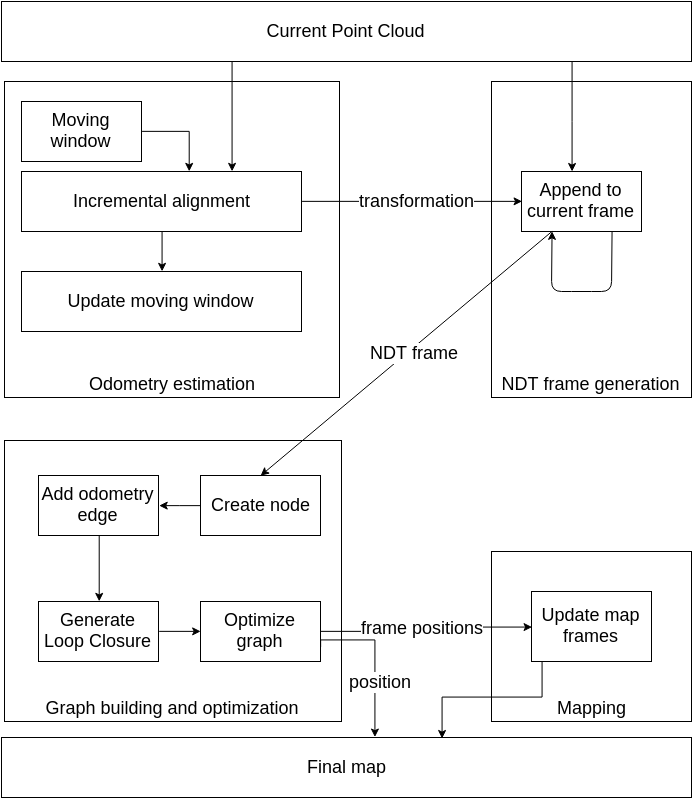
\includegraphics[width=100mm]{../img/algorithm_runtime.png}
	\caption{Diagram of graph based SLAM on NDT maps}
	\label{fig:algorithm}
\end{figure}
  
\newpage


\section{Moving window}
\label{sec:window}
Moving window is a special type of \gls{NDT} grid. It uses all features of \gls{NDT-OM} including occupancy update and dynamic object rejection. In addition, it offers way of moving window based on movement of a robot. Main idea behind moving window is to offer small map which can be used by incremental scanmatcher in order to efficiently align incoming scans against longer history. In standard incremental scanmatching approaches we need to know whole map. Information from whole map is used to correct small errors  when revisiting same place. A problem with this method arise when alignment fails. In this case wrongly aligned scan is merged into the map. This creates same place in the map twice. This can be wrongly understood by next registration and error might be never corrected. \gls{NDT-OM} can solve some of degeneration be cleaning occupied cells which are on the way between robot position and new measurement. In order for this mechanism to work next alignment scan needs to converge to original correct position. This is very unlikely with already corrupted map.

In our system we do not need to know whole map of environment because loops closures errors are fixed by graph optimization. We need incremental scanmatcher to provide us good estimate of robot movement. For this purpose we only need to know the part of environment occupied by current scan. It strongly depends on the type of sensor and environment. In our experiments, robot operated in indoor environment with laser sensor ranging up to 20m in long corridors. We have selected window radius of 15m which has provided the best compromise between speed ,memory and alignment efficiency. 

Size of windows also affects speed of recovering from alignment errors. Larger window holds information about bigger area. For single point in the window robot needs to travel up to length of the window. Smaller windows also reflect faster changes in the environment.

To prevent any alignment issues we decided to perform fast scanmatching. This means process most of the data from laser. High frequency scanmatching does not need initial guess because valid result is reasonably close.  Registration algorithm capable of this performance needs to work in order of milliseconds. We have experimented with three different algorithms. First one is \gls{P2D}-\gls{NDT} algorithm described in \ref{subsec:P2D_NDT}. Than we have experimented with same algorithm but with limited input cloud. We have constructed \gls{NDT} grid out of original cloud. All cells with valid means were changed into point cloud. Each cell was represented by its mean value. By doing this we have reduced number of points and increase speed of \gls{P2D}-NDT. Third algorithm is \gls{D2D}-\gls{NDT} described in \ref{subsec:D2D_NDT}. 






- what it is
- how is it updated
- why we have limited size
- wy size metters
-  what happens if underliieng graph changes
- visualization of running window
- registration method selection -results
- 
\newpage

\section{NDT frame}
\label{sec:NDT_frame}
- decriptions or creation
- why we dont input every measurement by it sefl to graph / why we need it
- visualization
- updating position
\newpage

\section{(Robust D2D-NDT registration)}
\label{sec:Robust D2D-NDT}

\subsection{Results}
\newpage

\newpage
\section{Loop closure detection}
\label{sec:LoopClosureMetric}
- loop closure detection metric
- radius search explained
\newpage